\documentclass[10pt,twocolumn,letterpaper]{article}
% ICCV Rules:
% 8 page limit (6 free + 2 paid)
% 10MB pdf file size limit
% 30MB supplementary materials file size limit (PDF or ZIP)

\usepackage{iccv}
\usepackage{times}
\usepackage{epsfig}
\usepackage{graphicx}
\usepackage{amsmath}
\usepackage{amssymb}

% Packages added by us
\usepackage{amsfonts}
\usepackage{mydefs}
\usepackage{algorithmic}
\usepackage{algorithm}

\usepackage[pagebackref=true,breaklinks=true,letterpaper=true,colorlinks,bookmarks=false]{hyperref}


% Needed for getting formulas in dia diagrams.
\usepackage{pstricks}
\usepackage{tikz}

% \cvprfinalcopy % *** Uncomment this line for the final submission

\def\iccvPaperID{257} % *** Enter the CVPR Paper ID here
\def\httilde{\mbox{\tt\raisebox{-.5ex}{\symbol{126}}}}

% Pages are numbered in submission mode, and unnumbered in camera-ready
\ificcvfinal\pagestyle{empty}\fi
\begin{document}

%\title{Accelerating $\ell_1$-Minimization Using Many-Core CPUs/GPUs \\ and Application to Face Recognition
%\title{Efficient Parallelization of Sparse Representation for Face Recognition}
%\thanks{Corresponding author: . This work was partially supported by ARO MURI W911NF-06-1-0076.}}
%\title{Many-Core Parallelization of $\ell_1$-Minimization for Face Recognition
\title{Parallelization of Fast $\ell_1$-Minimization for Face Recognition
%\thanks{Corresponding author: . This work was partially supported by ARO MURI W911NF-06-1-0076.}
}

\author{First Author\\
Institution1\\
Institution1 address\\
{\tt\small firstauthor@i1.org}
% For a paper whose authors are all at the same institution,
% omit the following lines up until the closing ``}''.
% Additional authors and addresses can be added with ``\and'',
% just like the second author.
% To save space, use either the email address or home page, not both
\and
Second Author\\
Institution2\\
First line of institution2 address\\
{\small\url{http://www.author.org/~second}}
}

\maketitle

\begin{abstract}

\end{abstract}

\section{Introduction} 
$\ell_1$-minimization ($\ell_1$-min) has received much attention in recent
years due to important applications in compressive sensing
\cite{BrucksteinA2007} and sparse representation \cite{WrightJ2010-PIEEE}.  
$\ell_1$-min refers to finding the minimum $\ell$-norm solution to an
underdetermined linear system $\bb=A\xx$:
\begin{equation}
\min \|\xx\|_1\quad \mbox{ subj. to }\quad \bb = A\xx.
\label{eq:l1min}
\end{equation}
It is now well established that, under certain conditions
\cite{CandesE2005-IT_1,DonohoD2004}, the minimum $\ell_1$-norm solution is also
the \emph{sparsest} solution to the system \eqref{eq:l1min}.

Among its many applications, $\ell_1$-min has been recently used to reformulate
image-based face recognition as a sparse representation problem
\cite{WrightJ2009-PAMI}.  If we stack the training images of $K$ subject
classes $(A_1\in\Re^{d\times n_1}, \cdots, A_K\in\Re^{d\times n_K})$ into the
columns of a matrix $A = [A_1, \cdots, A_K]\in\Re^{d\times n}$, given a new
query image in the same vector form $\bb\in\Re^d$, \emph{sparsity-based
classification} (SBC) solves the following minimization problem:
\begin{equation}
\min_{\xx, \ee} \| \xx \|_1 + \|\ee\|_1 \quad \subj \quad \bb = A \xx + \ee.
\label{eq:l1min_denoise}
\end{equation}
If the sparsest solutions for $\x$ and $\e$ are recovered, $\ee$ provides a
means to compensate for pixels that are corrupted due to occlusion of some part of the query
image, and the dominant nonzero coefficients of $\xx$ reveal the membership of
$\bb$ based on the training image labels associated with $A$.  Since $A$ ideally
contains many images per user taken under different illuminations, 
$A\x$ also acts as a linear illumination model for the test image $\bb$.

In this paper, we study parallelization of $\ell$-min on many-core CPU and GPU
architectures. Although $\ell_1$-min \eqref{eq:l1min} is a convex
program, conventional algorithms such as interior-point methods
\cite{ChenS2001-SIAM,TibshiraniR1996} are known to suffer from poor scalability
for large-scale applications such as face recognition. Recently, a number of
accelerated algorithms have been proposed that explicitly take advantage of
the special structure of $\ell_1$-min problems
\cite{LorisI2009,YangA2010-ICIP}. We investigate parallelization of a
state-of-the-art $\ell_1$-min solution based on the classical framework of
\emph{augmented Lagrange multiplier} (ALM) \cite{BertsekasD2003,YangA2010-ICIP}.

While solving \eqref{eq:l1min_denoise} can achieve exceptional
recognition accuracy on public databases, its success relies on the assumption
that the query image is well aligned with the training images. In
\cite{WagnerA2009-CVPR}, the framework of SBC was extended to iteratively align
a query image to one subject class. The face alignment algorithm in turn solves
the following minimization problem:
\begin{equation}
\hat{\tau}_i = \arg\min_{\xx, \ee, \tau_i} \|\ee\|_1\quad \mbox{subj. to}\quad \tilde\bb\circ\tau_i = A_i\xx + \ee,
\label{eq:l1min_alignment}
\end{equation}
where $\tau_i\in T$ is in a finite-dimensional group $T$ of transformations
(e.g., affine or homography) acting on the image domain, which aligns $\tilde\bb$
with the training images from the $i$-th class $A_i$. The algorithm 
extends Lucas-Kanade iterative alignment \cite{LucasB1981} to both to use the
$\ell_1$ norm as a robust error function, and also simultaneously 
to estimate the illumination model $A\x$.  
The original solution \cite{WagnerA2009-CVPR} was implemented based 
on standard interior-point
methods, and its speed has been since improved by ALM in a more recent paper
\cite{WagnerA2011-PAMI}. However, primarily due the high per-user cost
of the alignment step, the recognition system was still not fast enough
for real-time recognition against datasets of hundreds of users.
In this paper, in addition to solving the generic
$\ell_1$-min objectives \eqref{eq:l1min} and \eqref{eq:l1min_denoise}, we 
discuss how to properly accelerate the iterative face alignment step
\eqref{eq:l1min_alignment} on multi-core CPUs and GPUs. 

Finally, we present extensive benchmark to compare the performance of the
generic ALM $\ell_1$-min algorithm and the corresponding face recognition
routines on massively parallel CPUs and GPUs.  To this end, the face
recognition system has been fully implemented on a state-of-the-art
workstation, as shown in Figure \ref{fig:pipeline}. 
Since the parallelization of any algorithm
is highly dependent on the target hardware, we will give a brief overview of
the architecture of our test system in detail in Section
\ref{sec:parallelism}.  We will show that a highly accurate and robust face
recognition system can be constructed to recognize face images from a 
database of several hundred subjects quickly enough to be practical for
access control applications. 
Note that for applications targeting thousands of users or more, it would likely be
necessary to distribute the work over a network of machines; this paper
focuses on the (shared memory) parallelism available in a single machine.
The C++ source code of our implementations, which target Nvidia's CUDA GPU architecture
will be made available for evaluation by other researchers.
\begin{figure}
\centering
{\tiny % Graphic for TeX using PGF
% Title: pipeline_simplified.dia
% Creator: Dia v0.97-pre3
% CreationDate: Mon Feb 14 03:20:49 2011
% For: awagner
% \usepackage{tikz}
% The following commands are not supported in PSTricks at present
% We define them conditionally, so when they are implemented,
% this pgf file will use them.
\ifx\du\undefined
  \newlength{\du}
\fi
\setlength{\du}{15\unitlength}
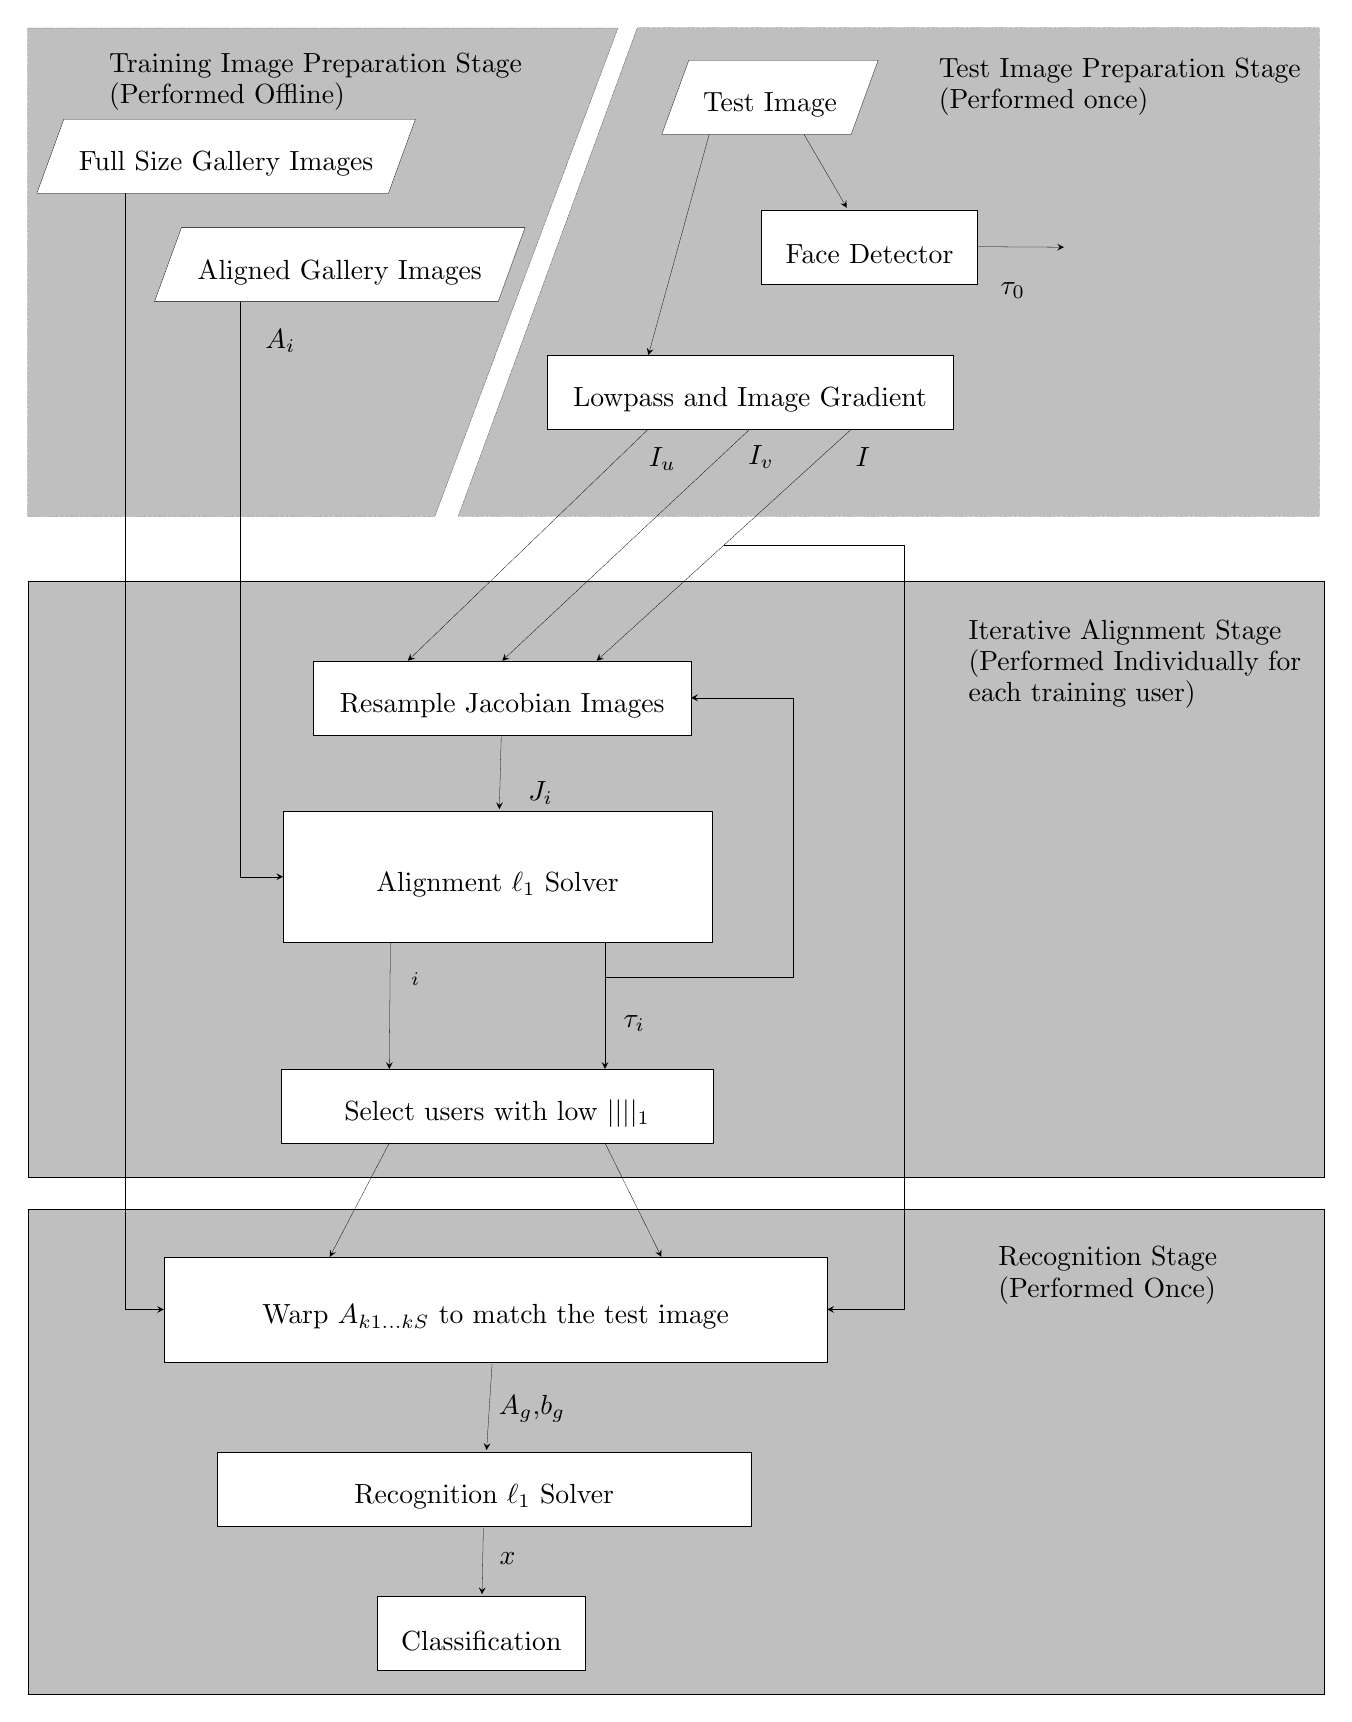
\begin{tikzpicture}
\pgftransformxscale{0.494667}
\pgftransformyscale{-0.494667}
\definecolor{dialinecolor}{rgb}{0.000000, 0.000000, 0.000000}
\pgfsetstrokecolor{dialinecolor}
\definecolor{dialinecolor}{rgb}{1.000000, 1.000000, 1.000000}
\pgfsetfillcolor{dialinecolor}
% setfont left to latex
\definecolor{dialinecolor}{rgb}{0.000000, 0.000000, 0.000000}
\pgfsetstrokecolor{dialinecolor}
\node[anchor=west] at (24.925000\du,42.952500\du){};
% setfont left to latex
\definecolor{dialinecolor}{rgb}{0.000000, 0.000000, 0.000000}
\pgfsetstrokecolor{dialinecolor}
\node[anchor=west] at (24.925000\du,42.952500\du){};
% setfont left to latex
\definecolor{dialinecolor}{rgb}{0.000000, 0.000000, 0.000000}
\pgfsetstrokecolor{dialinecolor}
\node[anchor=west] at (24.925000\du,42.952500\du){};
\definecolor{dialinecolor}{rgb}{0.749020, 0.749020, 0.749020}
\pgfsetfillcolor{dialinecolor}
\fill (6.494040\du,27.943300\du)--(6.494040\du,43.255071\du)--(39.770015\du,43.255071\du)--(39.770015\du,27.943300\du)--cycle;
\pgfsetlinewidth{0.100000\du}
\pgfsetdash{{\pgflinewidth}{0.200000\du}}{0cm}
\pgfsetdash{{\pgflinewidth}{0.200000\du}}{0cm}
\pgfsetmiterjoin
\definecolor{dialinecolor}{rgb}{0.000000, 0.000000, 0.000000}
\pgfsetstrokecolor{dialinecolor}
\draw (6.494040\du,27.943300\du)--(6.494040\du,43.255071\du)--(39.770015\du,43.255071\du)--(39.770015\du,27.943300\du)--cycle;
% setfont left to latex
\definecolor{dialinecolor}{rgb}{0.000000, 0.000000, 0.000000}
\pgfsetstrokecolor{dialinecolor}
\node at (23.132027\du,35.794186\du){};
\definecolor{dialinecolor}{rgb}{0.749020, 0.749020, 0.749020}
\pgfsetfillcolor{dialinecolor}
\fill (6.494040\du,44.061200\du)--(6.494040\du,56.519596\du)--(39.770015\du,56.519596\du)--(39.770015\du,44.061200\du)--cycle;
\pgfsetlinewidth{0.100000\du}
\pgfsetdash{{\pgflinewidth}{0.200000\du}}{0cm}
\pgfsetdash{{\pgflinewidth}{0.200000\du}}{0cm}
\pgfsetmiterjoin
\definecolor{dialinecolor}{rgb}{0.000000, 0.000000, 0.000000}
\pgfsetstrokecolor{dialinecolor}
\draw (6.494040\du,44.061200\du)--(6.494040\du,56.519596\du)--(39.770015\du,56.519596\du)--(39.770015\du,44.061200\du)--cycle;
% setfont left to latex
\definecolor{dialinecolor}{rgb}{0.000000, 0.000000, 0.000000}
\pgfsetstrokecolor{dialinecolor}
\node at (23.132027\du,50.485398\du){};
% setfont left to latex
\definecolor{dialinecolor}{rgb}{0.000000, 0.000000, 0.000000}
\pgfsetstrokecolor{dialinecolor}
\node[anchor=west] at (23.132000\du,35.599200\du){};
% setfont left to latex
\definecolor{dialinecolor}{rgb}{0.000000, 0.000000, 0.000000}
\pgfsetstrokecolor{dialinecolor}
\node[anchor=west] at (23.132000\du,35.599200\du){};
% setfont left to latex
\definecolor{dialinecolor}{rgb}{0.000000, 0.000000, 0.000000}
\pgfsetstrokecolor{dialinecolor}
\node[anchor=west] at (30.406100\du,29.259100\du){Iterative Alignment Stage};
% setfont left to latex
\definecolor{dialinecolor}{rgb}{0.000000, 0.000000, 0.000000}
\pgfsetstrokecolor{dialinecolor}
\node[anchor=west] at (30.406100\du,30.059100\du){(Performed Individually for};
% setfont left to latex
\definecolor{dialinecolor}{rgb}{0.000000, 0.000000, 0.000000}
\pgfsetstrokecolor{dialinecolor}
\node[anchor=west] at (30.406100\du,30.859100\du){each training user)};
% setfont left to latex
\definecolor{dialinecolor}{rgb}{0.000000, 0.000000, 0.000000}
\pgfsetstrokecolor{dialinecolor}
\node[anchor=west] at (31.173700\du,45.350700\du){Recognition Stage};
% setfont left to latex
\definecolor{dialinecolor}{rgb}{0.000000, 0.000000, 0.000000}
\pgfsetstrokecolor{dialinecolor}
\node[anchor=west] at (31.173700\du,46.150700\du){(Performed Once)};
\pgfsetlinewidth{0.100000\du}
\pgfsetdash{{\pgflinewidth}{0.200000\du}}{0cm}
\pgfsetdash{{\pgflinewidth}{0.200000\du}}{0cm}
\pgfsetmiterjoin
\pgfsetbuttcap
\definecolor{dialinecolor}{rgb}{0.749020, 0.749020, 0.749020}
\pgfsetfillcolor{dialinecolor}
\fill (6.494040\du,13.746400\du)--(21.645100\du,13.746400\du)--(16.943000\du,26.285100\du)--(6.494040\du,26.285100\du)--cycle;
\definecolor{dialinecolor}{rgb}{0.000000, 0.000000, 0.000000}
\pgfsetstrokecolor{dialinecolor}
\draw (6.494040\du,13.746400\du)--(21.645100\du,13.746400\du)--(16.943000\du,26.285100\du)--(6.494040\du,26.285100\du)--cycle;
% setfont left to latex
\definecolor{dialinecolor}{rgb}{0.000000, 0.000000, 0.000000}
\pgfsetstrokecolor{dialinecolor}
\node[anchor=west] at (8.342710\du,14.710900\du){Training Image Preparation Stage};
% setfont left to latex
\definecolor{dialinecolor}{rgb}{0.000000, 0.000000, 0.000000}
\pgfsetstrokecolor{dialinecolor}
\node[anchor=west] at (8.342710\du,15.510900\du){(Performed Offline)};
\pgfsetlinewidth{0.100000\du}
\pgfsetdash{{\pgflinewidth}{0.200000\du}}{0cm}
\pgfsetdash{{\pgflinewidth}{0.200000\du}}{0cm}
\pgfsetmiterjoin
\pgfsetbuttcap
\definecolor{dialinecolor}{rgb}{0.749020, 0.749020, 0.749020}
\pgfsetfillcolor{dialinecolor}
\fill (22.141100\du,13.740100\du)--(39.649500\du,13.740100\du)--(39.649500\du,26.278900\du)--(17.545800\du,26.278900\du)--cycle;
\definecolor{dialinecolor}{rgb}{0.000000, 0.000000, 0.000000}
\pgfsetstrokecolor{dialinecolor}
\draw (22.141100\du,13.740100\du)--(39.649500\du,13.740100\du)--(39.649500\du,26.278900\du)--(17.545800\du,26.278900\du)--cycle;
% setfont left to latex
\definecolor{dialinecolor}{rgb}{0.000000, 0.000000, 0.000000}
\pgfsetstrokecolor{dialinecolor}
\node[anchor=west] at (29.642500\du,14.831400\du){Test Image Preparation Stage};
% setfont left to latex
\definecolor{dialinecolor}{rgb}{0.000000, 0.000000, 0.000000}
\pgfsetstrokecolor{dialinecolor}
\node[anchor=west] at (29.642500\du,15.631400\du){(Performed once)};
\definecolor{dialinecolor}{rgb}{1.000000, 1.000000, 1.000000}
\pgfsetfillcolor{dialinecolor}
\fill (23.464443\du,14.572100\du)--(28.325620\du,14.572100\du)--(27.634076\du,16.472100\du)--(22.772900\du,16.472100\du)--cycle;
\pgfsetlinewidth{0.100000\du}
\pgfsetdash{}{0pt}
\pgfsetdash{}{0pt}
\pgfsetmiterjoin
\definecolor{dialinecolor}{rgb}{0.000000, 0.000000, 0.000000}
\pgfsetstrokecolor{dialinecolor}
\draw (23.464443\du,14.572100\du)--(28.325620\du,14.572100\du)--(27.634076\du,16.472100\du)--(22.772900\du,16.472100\du)--cycle;
% setfont left to latex
\definecolor{dialinecolor}{rgb}{0.000000, 0.000000, 0.000000}
\pgfsetstrokecolor{dialinecolor}
\node at (25.549260\du,15.717100\du){Test Image};
\definecolor{dialinecolor}{rgb}{1.000000, 1.000000, 1.000000}
\pgfsetfillcolor{dialinecolor}
\fill (13.826900\du,29.990700\du)--(13.826900\du,31.890700\du)--(23.521900\du,31.890700\du)--(23.521900\du,29.990700\du)--cycle;
\pgfsetlinewidth{0.100000\du}
\pgfsetdash{}{0pt}
\pgfsetdash{}{0pt}
\pgfsetmiterjoin
\definecolor{dialinecolor}{rgb}{0.000000, 0.000000, 0.000000}
\pgfsetstrokecolor{dialinecolor}
\draw (13.826900\du,29.990700\du)--(13.826900\du,31.890700\du)--(23.521900\du,31.890700\du)--(23.521900\du,29.990700\du)--cycle;
% setfont left to latex
\definecolor{dialinecolor}{rgb}{0.000000, 0.000000, 0.000000}
\pgfsetstrokecolor{dialinecolor}
\node at (18.674400\du,31.135700\du){Resample Jacobian Images};
\definecolor{dialinecolor}{rgb}{1.000000, 1.000000, 1.000000}
\pgfsetfillcolor{dialinecolor}
\fill (13.050000\du,33.850000\du)--(13.050000\du,37.221200\du)--(24.058800\du,37.221200\du)--(24.058800\du,33.850000\du)--cycle;
\pgfsetlinewidth{0.100000\du}
\pgfsetdash{}{0pt}
\pgfsetdash{}{0pt}
\pgfsetmiterjoin
\definecolor{dialinecolor}{rgb}{0.000000, 0.000000, 0.000000}
\pgfsetstrokecolor{dialinecolor}
\draw (13.050000\du,33.850000\du)--(13.050000\du,37.221200\du)--(24.058800\du,37.221200\du)--(24.058800\du,33.850000\du)--cycle;
% setfont left to latex
\definecolor{dialinecolor}{rgb}{0.000000, 0.000000, 0.000000}
\pgfsetstrokecolor{dialinecolor}
\node at (18.554400\du,35.730600\du){Alignment $\ell_1$ Solver};
\pgfsetlinewidth{0.100000\du}
\pgfsetdash{}{0pt}
\pgfsetdash{}{0pt}
\pgfsetbuttcap
{
\definecolor{dialinecolor}{rgb}{0.000000, 0.000000, 0.000000}
\pgfsetfillcolor{dialinecolor}
% was here!!!
\pgfsetarrowsend{stealth}
\definecolor{dialinecolor}{rgb}{0.000000, 0.000000, 0.000000}
\pgfsetstrokecolor{dialinecolor}
\draw (18.648326\du,31.939104\du)--(18.599693\du,33.801294\du);
}
% setfont left to latex
\definecolor{dialinecolor}{rgb}{0.000000, 0.000000, 0.000000}
\pgfsetstrokecolor{dialinecolor}
\node[anchor=west] at (11.250000\du,34.890000\du){};
\definecolor{dialinecolor}{rgb}{1.000000, 1.000000, 1.000000}
\pgfsetfillcolor{dialinecolor}
\fill (19.817600\du,22.143000\du)--(19.817600\du,24.043000\du)--(30.250100\du,24.043000\du)--(30.250100\du,22.143000\du)--cycle;
\pgfsetlinewidth{0.100000\du}
\pgfsetdash{}{0pt}
\pgfsetdash{}{0pt}
\pgfsetmiterjoin
\definecolor{dialinecolor}{rgb}{0.000000, 0.000000, 0.000000}
\pgfsetstrokecolor{dialinecolor}
\draw (19.817600\du,22.143000\du)--(19.817600\du,24.043000\du)--(30.250100\du,24.043000\du)--(30.250100\du,22.143000\du)--cycle;
% setfont left to latex
\definecolor{dialinecolor}{rgb}{0.000000, 0.000000, 0.000000}
\pgfsetstrokecolor{dialinecolor}
\node at (25.033850\du,23.288000\du){Lowpass and Image Gradient};
\definecolor{dialinecolor}{rgb}{1.000000, 1.000000, 1.000000}
\pgfsetfillcolor{dialinecolor}
\fill (25.332900\du,18.409900\du)--(25.332900\du,20.309900\du)--(30.875400\du,20.309900\du)--(30.875400\du,18.409900\du)--cycle;
\pgfsetlinewidth{0.100000\du}
\pgfsetdash{}{0pt}
\pgfsetdash{}{0pt}
\pgfsetmiterjoin
\definecolor{dialinecolor}{rgb}{0.000000, 0.000000, 0.000000}
\pgfsetstrokecolor{dialinecolor}
\draw (25.332900\du,18.409900\du)--(25.332900\du,20.309900\du)--(30.875400\du,20.309900\du)--(30.875400\du,18.409900\du)--cycle;
% setfont left to latex
\definecolor{dialinecolor}{rgb}{0.000000, 0.000000, 0.000000}
\pgfsetstrokecolor{dialinecolor}
\node at (28.104150\du,19.554900\du){Face Detector};
\definecolor{dialinecolor}{rgb}{1.000000, 1.000000, 1.000000}
\pgfsetfillcolor{dialinecolor}
\fill (9.987950\du,45.295200\du)--(9.987950\du,47.995200\du)--(27.017950\du,47.995200\du)--(27.017950\du,45.295200\du)--cycle;
\pgfsetlinewidth{0.100000\du}
\pgfsetdash{}{0pt}
\pgfsetdash{}{0pt}
\pgfsetmiterjoin
\definecolor{dialinecolor}{rgb}{0.000000, 0.000000, 0.000000}
\pgfsetstrokecolor{dialinecolor}
\draw (9.987950\du,45.295200\du)--(9.987950\du,47.995200\du)--(27.017950\du,47.995200\du)--(27.017950\du,45.295200\du)--cycle;
% setfont left to latex
\definecolor{dialinecolor}{rgb}{0.000000, 0.000000, 0.000000}
\pgfsetstrokecolor{dialinecolor}
\node at (18.502950\du,46.840200\du){Warp $A_{k1 \ldots kS}$ to match the test image};
\definecolor{dialinecolor}{rgb}{1.000000, 1.000000, 1.000000}
\pgfsetfillcolor{dialinecolor}
\fill (15.470400\du,54.006500\du)--(15.470400\du,55.906500\du)--(20.802900\du,55.906500\du)--(20.802900\du,54.006500\du)--cycle;
\pgfsetlinewidth{0.100000\du}
\pgfsetdash{}{0pt}
\pgfsetdash{}{0pt}
\pgfsetmiterjoin
\definecolor{dialinecolor}{rgb}{0.000000, 0.000000, 0.000000}
\pgfsetstrokecolor{dialinecolor}
\draw (15.470400\du,54.006500\du)--(15.470400\du,55.906500\du)--(20.802900\du,55.906500\du)--(20.802900\du,54.006500\du)--cycle;
% setfont left to latex
\definecolor{dialinecolor}{rgb}{0.000000, 0.000000, 0.000000}
\pgfsetstrokecolor{dialinecolor}
\node at (18.136650\du,55.151500\du){Classification};
% setfont left to latex
\definecolor{dialinecolor}{rgb}{0.000000, 0.000000, 0.000000}
\pgfsetstrokecolor{dialinecolor}
\node[anchor=west] at (28.104200\du,19.359900\du){};
\pgfsetlinewidth{0.100000\du}
\pgfsetdash{}{0pt}
\pgfsetdash{}{0pt}
\pgfsetbuttcap
{
\definecolor{dialinecolor}{rgb}{0.000000, 0.000000, 0.000000}
\pgfsetfillcolor{dialinecolor}
% was here!!!
\pgfsetarrowsend{stealth}
\definecolor{dialinecolor}{rgb}{0.000000, 0.000000, 0.000000}
\pgfsetstrokecolor{dialinecolor}
\draw (25.033800\du,24.043000\du)--(18.674400\du,29.990700\du);
}
\pgfsetlinewidth{0.100000\du}
\pgfsetdash{}{0pt}
\pgfsetdash{}{0pt}
\pgfsetbuttcap
{
\definecolor{dialinecolor}{rgb}{0.000000, 0.000000, 0.000000}
\pgfsetfillcolor{dialinecolor}
% was here!!!
\pgfsetarrowsend{stealth}
\definecolor{dialinecolor}{rgb}{0.000000, 0.000000, 0.000000}
\pgfsetstrokecolor{dialinecolor}
\draw (22.425700\du,24.043000\du)--(16.250600\du,29.990700\du);
}
\pgfsetlinewidth{0.100000\du}
\pgfsetdash{}{0pt}
\pgfsetdash{}{0pt}
\pgfsetbuttcap
{
\definecolor{dialinecolor}{rgb}{0.000000, 0.000000, 0.000000}
\pgfsetfillcolor{dialinecolor}
% was here!!!
\pgfsetarrowsend{stealth}
\definecolor{dialinecolor}{rgb}{0.000000, 0.000000, 0.000000}
\pgfsetstrokecolor{dialinecolor}
\draw (27.641900\du,24.043000\du)--(21.098100\du,29.990700\du);
}
% setfont left to latex
\definecolor{dialinecolor}{rgb}{0.000000, 0.000000, 0.000000}
\pgfsetstrokecolor{dialinecolor}
\node[anchor=west] at (27.506000\du,24.761200\du){$I$};
% setfont left to latex
\definecolor{dialinecolor}{rgb}{0.000000, 0.000000, 0.000000}
\pgfsetstrokecolor{dialinecolor}
\node[anchor=west] at (22.199300\du,24.802400\du){$I_u$};
\pgfsetlinewidth{0.100000\du}
\pgfsetdash{}{0pt}
\pgfsetdash{}{0pt}
\pgfsetbuttcap
{
\definecolor{dialinecolor}{rgb}{0.000000, 0.000000, 0.000000}
\pgfsetfillcolor{dialinecolor}
% was here!!!
\pgfsetarrowsend{stealth}
\definecolor{dialinecolor}{rgb}{0.000000, 0.000000, 0.000000}
\pgfsetstrokecolor{dialinecolor}
\draw (23.988200\du,16.472100\du)--(22.425700\du,22.143000\du);
}
\pgfsetlinewidth{0.100000\du}
\pgfsetdash{}{0pt}
\pgfsetdash{}{0pt}
\pgfsetbuttcap
{
\definecolor{dialinecolor}{rgb}{0.000000, 0.000000, 0.000000}
\pgfsetfillcolor{dialinecolor}
% was here!!!
\pgfsetarrowsend{stealth}
\definecolor{dialinecolor}{rgb}{0.000000, 0.000000, 0.000000}
\pgfsetstrokecolor{dialinecolor}
\draw (26.418800\du,16.472100\du)--(27.520491\du,18.359816\du);
}
% setfont left to latex
\definecolor{dialinecolor}{rgb}{0.000000, 0.000000, 0.000000}
\pgfsetstrokecolor{dialinecolor}
\node[anchor=west] at (28.248200\du,27.724100\du){};
% setfont left to latex
\definecolor{dialinecolor}{rgb}{0.000000, 0.000000, 0.000000}
\pgfsetstrokecolor{dialinecolor}
\node[anchor=west] at (31.230200\du,20.488200\du){$\tau_0$};
\definecolor{dialinecolor}{rgb}{1.000000, 1.000000, 1.000000}
\pgfsetfillcolor{dialinecolor}
\fill (7.418823\du,16.086600\du)--(16.445000\du,16.086600\du)--(15.753456\du,17.986600\du)--(6.727280\du,17.986600\du)--cycle;
\pgfsetlinewidth{0.100000\du}
\pgfsetdash{}{0pt}
\pgfsetdash{}{0pt}
\pgfsetmiterjoin
\definecolor{dialinecolor}{rgb}{0.000000, 0.000000, 0.000000}
\pgfsetstrokecolor{dialinecolor}
\draw (7.418823\du,16.086600\du)--(16.445000\du,16.086600\du)--(15.753456\du,17.986600\du)--(6.727280\du,17.986600\du)--cycle;
% setfont left to latex
\definecolor{dialinecolor}{rgb}{0.000000, 0.000000, 0.000000}
\pgfsetstrokecolor{dialinecolor}
\node at (11.586140\du,17.231600\du){Full Size Gallery Images};
\pgfsetlinewidth{0.100000\du}
\pgfsetdash{}{0pt}
\pgfsetdash{}{0pt}
\pgfsetmiterjoin
\pgfsetbuttcap
{
\definecolor{dialinecolor}{rgb}{0.000000, 0.000000, 0.000000}
\pgfsetfillcolor{dialinecolor}
% was here!!!
\pgfsetarrowsend{stealth}
{\pgfsetcornersarced{\pgfpoint{0.000000\du}{0.000000\du}}\definecolor{dialinecolor}{rgb}{0.000000, 0.000000, 0.000000}
\pgfsetstrokecolor{dialinecolor}
\draw (11.952169\du,20.770000\du)--(11.952169\du,35.535600\du)--(13.050000\du,35.535600\du);
}}
\pgfsetlinewidth{0.100000\du}
\pgfsetdash{}{0pt}
\pgfsetdash{}{0pt}
\pgfsetbuttcap
{
\definecolor{dialinecolor}{rgb}{0.000000, 0.000000, 0.000000}
\pgfsetfillcolor{dialinecolor}
% was here!!!
\pgfsetarrowsend{stealth}
\definecolor{dialinecolor}{rgb}{0.000000, 0.000000, 0.000000}
\pgfsetstrokecolor{dialinecolor}
\draw (30.875400\du,19.359900\du)--(33.098700\du,19.372700\du);
}
\definecolor{dialinecolor}{rgb}{1.000000, 1.000000, 1.000000}
\pgfsetfillcolor{dialinecolor}
\fill (11.356800\du,50.303600\du)--(11.356800\du,52.203600\du)--(25.061036\du,52.203600\du)--(25.061036\du,50.303600\du)--cycle;
\pgfsetlinewidth{0.100000\du}
\pgfsetdash{}{0pt}
\pgfsetdash{}{0pt}
\pgfsetmiterjoin
\definecolor{dialinecolor}{rgb}{0.000000, 0.000000, 0.000000}
\pgfsetstrokecolor{dialinecolor}
\draw (11.356800\du,50.303600\du)--(11.356800\du,52.203600\du)--(25.061036\du,52.203600\du)--(25.061036\du,50.303600\du)--cycle;
% setfont left to latex
\definecolor{dialinecolor}{rgb}{0.000000, 0.000000, 0.000000}
\pgfsetstrokecolor{dialinecolor}
\node at (18.208918\du,51.448600\du){Recognition $\ell_1$ Solver};
\pgfsetlinewidth{0.100000\du}
\pgfsetdash{}{0pt}
\pgfsetdash{}{0pt}
\pgfsetmiterjoin
\pgfsetbuttcap
{
\definecolor{dialinecolor}{rgb}{0.000000, 0.000000, 0.000000}
\pgfsetfillcolor{dialinecolor}
% was here!!!
\pgfsetarrowsend{stealth}
{\pgfsetcornersarced{\pgfpoint{0.000000\du}{0.000000\du}}\definecolor{dialinecolor}{rgb}{0.000000, 0.000000, 0.000000}
\pgfsetstrokecolor{dialinecolor}
\draw (21.306600\du,37.221200\du)--(21.306600\du,38.050000\du)--(21.312500\du,38.050000\du)--(21.312500\du,40.470000\du);
}}
\pgfsetlinewidth{0.100000\du}
\pgfsetdash{}{0pt}
\pgfsetdash{}{0pt}
\pgfsetbuttcap
{
\definecolor{dialinecolor}{rgb}{0.000000, 0.000000, 0.000000}
\pgfsetfillcolor{dialinecolor}
% was here!!!
\pgfsetarrowsend{stealth}
\definecolor{dialinecolor}{rgb}{0.000000, 0.000000, 0.000000}
\pgfsetstrokecolor{dialinecolor}
\draw (15.802200\du,37.221200\du)--(15.775000\du,40.470000\du);
}
% setfont left to latex
\definecolor{dialinecolor}{rgb}{0.000000, 0.000000, 0.000000}
\pgfsetstrokecolor{dialinecolor}
\node[anchor=west] at (16.096600\du,38.150600\du){$\e_i$};
\pgfsetlinewidth{0.100000\du}
\pgfsetdash{}{0pt}
\pgfsetdash{}{0pt}
\pgfsetbuttcap
{
\definecolor{dialinecolor}{rgb}{0.000000, 0.000000, 0.000000}
\pgfsetfillcolor{dialinecolor}
% was here!!!
\pgfsetarrowsend{stealth}
\definecolor{dialinecolor}{rgb}{0.000000, 0.000000, 0.000000}
\pgfsetstrokecolor{dialinecolor}
\draw (18.189395\du,52.253907\du)--(18.156173\du,53.956193\du);
}
\pgfsetlinewidth{0.100000\du}
\pgfsetdash{}{0pt}
\pgfsetdash{}{0pt}
\pgfsetmiterjoin
\pgfsetbuttcap
{
\definecolor{dialinecolor}{rgb}{0.000000, 0.000000, 0.000000}
\pgfsetfillcolor{dialinecolor}
% was here!!!
\pgfsetarrowsend{stealth}
{\pgfsetcornersarced{\pgfpoint{0.000000\du}{0.000000\du}}\definecolor{dialinecolor}{rgb}{0.000000, 0.000000, 0.000000}
\pgfsetstrokecolor{dialinecolor}
\draw (24.370000\du,27.016800\du)--(28.999500\du,27.016800\du)--(28.999500\du,46.645200\du)--(27.018000\du,46.645200\du);
}}
\pgfsetlinewidth{0.100000\du}
\pgfsetdash{}{0pt}
\pgfsetdash{}{0pt}
\pgfsetbuttcap
{
\definecolor{dialinecolor}{rgb}{0.000000, 0.000000, 0.000000}
\pgfsetfillcolor{dialinecolor}
% was here!!!
\pgfsetarrowsend{stealth}
\definecolor{dialinecolor}{rgb}{0.000000, 0.000000, 0.000000}
\pgfsetstrokecolor{dialinecolor}
\draw (18.413613\du,48.045384\du)--(18.272699\du,50.253951\du);
}
% setfont left to latex
\definecolor{dialinecolor}{rgb}{0.000000, 0.000000, 0.000000}
\pgfsetstrokecolor{dialinecolor}
\node[anchor=west] at (18.367000\du,53.041300\du){$x$};
% setfont left to latex
\definecolor{dialinecolor}{rgb}{0.000000, 0.000000, 0.000000}
\pgfsetstrokecolor{dialinecolor}
\node[anchor=west] at (18.349600\du,49.203000\du){$A_g$,$b_g$};
% setfont left to latex
\definecolor{dialinecolor}{rgb}{0.000000, 0.000000, 0.000000}
\pgfsetstrokecolor{dialinecolor}
\node[anchor=west] at (24.755000\du,24.750000\du){$I_v$};
% setfont left to latex
\definecolor{dialinecolor}{rgb}{0.000000, 0.000000, 0.000000}
\pgfsetstrokecolor{dialinecolor}
\node[anchor=west] at (12.355000\du,21.787500\du){$A_i$};
% setfont left to latex
\definecolor{dialinecolor}{rgb}{0.000000, 0.000000, 0.000000}
\pgfsetstrokecolor{dialinecolor}
\node[anchor=west] at (19.105000\du,33.387500\du){$J_i$};
\definecolor{dialinecolor}{rgb}{1.000000, 1.000000, 1.000000}
\pgfsetfillcolor{dialinecolor}
\fill (10.437793\du,18.870000\du)--(19.261470\du,18.870000\du)--(18.569926\du,20.770000\du)--(9.746250\du,20.770000\du)--cycle;
\pgfsetlinewidth{0.100000\du}
\pgfsetdash{}{0pt}
\pgfsetdash{}{0pt}
\pgfsetmiterjoin
\definecolor{dialinecolor}{rgb}{0.000000, 0.000000, 0.000000}
\pgfsetstrokecolor{dialinecolor}
\draw (10.437793\du,18.870000\du)--(19.261470\du,18.870000\du)--(18.569926\du,20.770000\du)--(9.746250\du,20.770000\du)--cycle;
% setfont left to latex
\definecolor{dialinecolor}{rgb}{0.000000, 0.000000, 0.000000}
\pgfsetstrokecolor{dialinecolor}
\node at (14.503860\du,20.015000\du){Aligned Gallery Images};
\pgfsetlinewidth{0.100000\du}
\pgfsetdash{}{0pt}
\pgfsetdash{}{0pt}
\pgfsetmiterjoin
\pgfsetbuttcap
{
\definecolor{dialinecolor}{rgb}{0.000000, 0.000000, 0.000000}
\pgfsetfillcolor{dialinecolor}
% was here!!!
\pgfsetarrowsend{stealth}
{\pgfsetcornersarced{\pgfpoint{0.000000\du}{0.000000\du}}\definecolor{dialinecolor}{rgb}{0.000000, 0.000000, 0.000000}
\pgfsetstrokecolor{dialinecolor}
\draw (8.983824\du,17.986600\du)--(8.983824\du,46.645200\du)--(9.987950\du,46.645200\du);
}}
\pgfsetlinewidth{0.100000\du}
\pgfsetdash{}{0pt}
\pgfsetdash{}{0pt}
\pgfsetmiterjoin
\pgfsetbuttcap
{
\definecolor{dialinecolor}{rgb}{0.000000, 0.000000, 0.000000}
\pgfsetfillcolor{dialinecolor}
% was here!!!
\pgfsetarrowsend{stealth}
{\pgfsetcornersarced{\pgfpoint{0.000000\du}{0.000000\du}}\definecolor{dialinecolor}{rgb}{0.000000, 0.000000, 0.000000}
\pgfsetstrokecolor{dialinecolor}
\draw (21.300000\du,38.100000\du)--(26.150000\du,38.100000\du)--(26.150000\du,30.940700\du)--(23.521900\du,30.940700\du);
}}
% setfont left to latex
\definecolor{dialinecolor}{rgb}{0.000000, 0.000000, 0.000000}
\pgfsetstrokecolor{dialinecolor}
\node[anchor=west] at (21.550000\du,39.300000\du){$\tau_i$};
\definecolor{dialinecolor}{rgb}{1.000000, 1.000000, 1.000000}
\pgfsetfillcolor{dialinecolor}
\fill (13.006200\du,40.470000\du)--(13.006200\du,42.370000\du)--(24.081200\du,42.370000\du)--(24.081200\du,40.470000\du)--cycle;
\pgfsetlinewidth{0.100000\du}
\pgfsetdash{}{0pt}
\pgfsetdash{}{0pt}
\pgfsetmiterjoin
\definecolor{dialinecolor}{rgb}{0.000000, 0.000000, 0.000000}
\pgfsetstrokecolor{dialinecolor}
\draw (13.006200\du,40.470000\du)--(13.006200\du,42.370000\du)--(24.081200\du,42.370000\du)--(24.081200\du,40.470000\du)--cycle;
% setfont left to latex
\definecolor{dialinecolor}{rgb}{0.000000, 0.000000, 0.000000}
\pgfsetstrokecolor{dialinecolor}
\node at (18.543700\du,41.615000\du){Select users with low $||\e||_1$};
\pgfsetlinewidth{0.100000\du}
\pgfsetdash{}{0pt}
\pgfsetdash{}{0pt}
\pgfsetbuttcap
{
\definecolor{dialinecolor}{rgb}{0.000000, 0.000000, 0.000000}
\pgfsetfillcolor{dialinecolor}
% was here!!!
\pgfsetarrowsend{stealth}
\definecolor{dialinecolor}{rgb}{0.000000, 0.000000, 0.000000}
\pgfsetstrokecolor{dialinecolor}
\draw (15.775000\du,42.370000\du)--(14.245500\du,45.295200\du);
}
\pgfsetlinewidth{0.100000\du}
\pgfsetdash{}{0pt}
\pgfsetdash{}{0pt}
\pgfsetbuttcap
{
\definecolor{dialinecolor}{rgb}{0.000000, 0.000000, 0.000000}
\pgfsetfillcolor{dialinecolor}
% was here!!!
\pgfsetarrowsend{stealth}
\definecolor{dialinecolor}{rgb}{0.000000, 0.000000, 0.000000}
\pgfsetstrokecolor{dialinecolor}
\draw (21.312500\du,42.370000\du)--(22.760500\du,45.295200\du);
}
\end{tikzpicture}
}
\caption{Overview of the face recognition pipeline.}
\label{fig:pipeline}
\end{figure}

\subsection{Literature Review} 
In this section, we briefly review the literature of $\ell_1$-min and existing
works on its parallelization.  Traditionally, $\ell_1$-min (or the so-called
basis pursuit (BP)) has been formulated as a linear program
\cite{ChenS2001-SIAM}. Several variations of the solution are also well known
in optimization, including a noisy approximation via quadratic programming
called the LASSO \cite{TibshiraniR1996} and truncated Newton interior-point
method (TNIPM) \cite{KimS2007}.

One of the drawbacks of most interior-point methods for $\ell_1$-min (including
BP, LASSO, and TNIPM) is that they require the solution sequence to follow an
interior path{\bf DW: Following the interior path is what made them faster than
traditional linear programming techniques that follow the edge of the feasible set;
does Homotopy actually go outside the feasible set?  Just want to check if this is
an accurate representation...}, which is often computationally expensive. To mitigate these
issues, an approach called \emph{Homotopy} has been studied to accelerate the
speed of $\ell_1$-min. Homotopy methods for recovering sparse signals were
first studied in the context of LASSO \cite{OsborneM2000}, which inspired a
solution to the \emph{forward stagewise linear regression} problem called LARS
\cite{EfronB2004}, and eventually led to the corresponding Homotopy algorithms
for BP in \cite{MalioutovD2005,DonohoD2006}.

Although Homotopy can be shown to exactly estimate BP when the solution is
sufficiently sparse \cite{DonohoD2006}, the algorithm still involves 
computationally expensive operations such as matrix-matrix multiplication and 
the solution of least-squares problems with varying $A$ matrices. 
In Section \ref{sec:ALM}, we contend
that ALM is a better choice among Homotopy and other existing $\ell_1$-min
solvers for implementation on many-core CPUs and GPUs. The ALM algorithm belongs to a
category of approximate $\ell_1$-min solutions called \emph{iterative
shrinkage-thresholding} (IST) method \cite{WrightS2008,BeckA2009}.
IST algorithms mainly involves elementary operations such as vector 
algebra and matrix-vector multiplication. Therefore,
when the dimension of the problem becomes high, IST-type algorithms are
particularly suitable for systems in parallel-computing environments. In
\cite{YangA2010-ICIP}, the authors further showed that, compared to other
IST-type algorithms, ALM is able to achieve good estimation accuracy comparable
to BP and Homotopy, while at the same time significantly improve the speed
compared to these exact $\ell_1$-min solutions. Due to these facts, in this
paper, we choose ALM as the core algorithm to implement the complete parallel
face recognition pipeline.

In terms of the past works in parallel $\ell_1$-min, the literature has been
limited, to the best of our knowledge. In \cite{BorghiA2010}, Borghi et al.
developed a special proximal gradient $\ell_1$-min algorithm based on
Moreau-Yosida regularization. In \cite{MurphyM2010}, Murphy et al. presented
parallel implementation of the l1-SPIRIT MRI reconstruction algorithm on NVidia
programmable GPUs.

\section{Augmented Lagrange Multiplier Method}
\label{sec:ALM}

For the completeness of the paper, in this section, we briefly describe the ALM
algorithm for $\ell_1$-min \eqref{eq:l1min} \cite{YangA2010-ICIP} and analyze
its complexity. Parallelization of ALM for face alignment and recognition will
be discussed in Section \ref{sec:alignment} and Section \ref{sec:recognition},
respectively.

Lagrange multiplier methods have been frequently used in convex programming to
eliminate equality constraints via adding a significant penalty term to the
cost function for infeasible points. ALM methods differ from other
penalty-based approaches by simultaneously estimating the optimal solution and
Lagrange multipliers in an iterative fashion.  For $\ell_1$-min, the augmented
Lagrange function is defined as: \begin{equation} L_\mu(\xx,\yy) = \|\xx\|_1 +
\yy^T(\bb - A\xx - \ee) + \frac{\mu}{2} \| \bb-A\xx-\ee \|_2^2, \end{equation}
where $\mu > 0$ is a constant that penalizes infeasibility and $\yy$ is a
vector of lagrange multipliers.

In Lagrange Multiplier Theory, if there exists a Lagrangian $y^*$ that
satisfies the second-order sufficiency conditions for optimality
\cite{BertsekasD2003}, then for a sufficiently large $mu$, the optimal
$\ell_1$-min solution also minimizes
\begin{equation}
\xx^* = \arg \min L_\mu(\xx,\yy^*).
\label{eq:optimal-ALM}
\end{equation}

In practice, the optimal values for the triplet $(\xx^*, \yy^*, \uu)$ are all
unknown. Furthermore, it has been observed that if solving
\eqref{eq:optimal-ALM} with a large initial value of $\mu$ tends to lead to
slower convergence speed \cite{WrightS2008,YangA2010-ICIP}. In
\cite{BertsekasD2003,YangJ2009}, an alternating procedure has been proposed to
iteratively update $\xx$ and $\yy$:
\begin{equation}
\left \{
\begin{array}{lll}
\xx_{k+1} & = & \arg\min_{\xx} \, L_{\mu_k} (\xx,\yy_k)\\
\yy_{k+1} & = & \yy_k + \mu_k (\bb - A\xx_{k+1}) \\
\end{array}
\right . ,
\label{eq:alm}
\end{equation}
where $\left\{\mu_{k}\right\}$ is a monotonically increasing positive sequence.
The iteration terminates when the estimates $(\xx, \yy)$ converges.

Note that in the iterative procedure outlined in \eqref{eq:alm}, the second
step only involves vector algebra and matrix-vector multiplication. Therefore,
the procedure is computationally efficient only if it is easier to minimize the
augmented Lagrange function compared to solving the original problem
\eqref{eq:l1min} directly. In fact, the first step that minimizes $L_{\mu_k}
(\xx,\yy_k)$ assuming $\yy_k$ and $\mu_k$ are fixed can be solved element-wise
iteratively by a soft-thresholding algorithm \cite{WrightS2008,BeckA2009},
whose time complexity is bounded by $O(n^2)$ and can be easily parallelized.
Algorithm \ref{alg:alm} summarizes the ALM $\ell_1$-min algorithm.

 \begin{algorithm}[h]
\caption{Augmented Lagrange Multiplier (ALM)}
{\bf INPUT:} $\bb \in \Re^m$, $A \in \Re^{m \times n}$, $\tau\leftarrow$ largest eigenvalue of $A^TA$, and a constant $\rho>1$.
\begin{algorithmic}[1]
\WHILE{not converged ($k = 1,2,\ldots$)} \STATE $t_1 \leftarrow 1$, $\zz_1
\leftarrow \xx_k$, $\uu_1 \leftarrow \xx_k$ \WHILE{not
converged ($l = 1,2,\ldots$)} \STATE $\uu_{l+1}  \leftarrow
\mathrm{soft}\left(\zz_l - \frac{1}{\tau}A^T\left(A\zz_l - \bb
- \frac{1}{\mu_k}\yy_k\right), \frac{1}{\mu_k\tau}\right)$
\STATE $t_{l+1} \leftarrow \frac{1}{2}\left( 1 +
\sqrt{1+4t_l^2}\right)$ \STATE $\zz_{l+1} \leftarrow \uu_{l+1}
+ \frac{t_l - 1}{t_{l+1}}(\uu_{l+1} - \uu_l)$ \ENDWHILE \STATE$
\xx_{k+1} \leftarrow \uu_{l+1}$ \STATE $\yy_{k+1} \leftarrow
\yy_k + \mu_k (\bb - A\xx_{k+1})$ \STATE $\mu_{k+1} \leftarrow
\rho\cdot\mu_k$ \ENDWHILE 
\end{algorithmic}

{\bf OUTPUT:} $\xx^* \leftarrow \xx_k$.
\label{alg:alm}
\end{algorithm}

\section{Hardware Parallelism} \label{sec:parallelism} 
In this section we discuss the hardware architectures used in this paper. Aside
from the $\ell_1$-min algorithm, our choice of the architectures plays a
significant role in many practical decisions we make in Section
\ref{sec:alignment} and Section \ref{sec:recognition}.  For CPU implementation,
the system would make use of all the cores in as many CPUs are present on one
motherboard.  For GPU implementation, the system would make the best use of a
single many-core Nvidia GPU chip  on a PCI card (GPUs are commonly shipped with
a single GPU chip per PCI-express card).  Unless otherwise specified, all
implementations utilize single precision floating point datatypes.  

\subsection{CPU Hardware Parallelism} 
The baseline architecture for our experiments is a Linux workstation with two
quad-core Intel Nehalem E5530 processors clocked at 2.4 GHz.  Each processor
has its own memory interface, and is directly connected to half of the RAM
installed in the machine.  The amount of RAM installed exceeds the amount used
by the algorithms, and is not an important performance consideration.  

Each core has a 32\,KB L1 data cache and a 256\,KB L2 cache. With Hyperthreading
enabled, each core can support two threads simultaneously.  For floating point
instructions, each core also has a vector unit capable of performing the same
arithmetic operation on four single precision floating point values
simultaneously.  \footnote{The core also has scalar floating point units, but
some compilers, notably gcc, generate code that uses the vector units
exclusively for floating point instructions.} 

There are thus two important levels of parallelism that need to be exploited to
efficiently use a modern CPU: core-level parallelism and vector-level
parallelism.  For the implementations discussed here, we will primarily use the
OpenMP programming model to express core-level parallelism {\bf AY: What is
OpenMP? citation needed}.  Depending on the section of the code{\bf AY: What is
a section of the code?}, we will achieve vector-level parallelism implicitly
through either the auto-vectorization features of Intel's icc compiler, or
through the use of a highly optimized BLAS library (Intel's MKL). {\bf AY:
citations needed, what is icc, what is the relation between BLAS and MKL? Are
they equivalent? not clear in the context.}

Each processor further has 8MB of L3 cache that is shared by all four cores.
Overall, this means the algorithm has approximately 16MB of on-chip cache
available.  For the low resolution images used in sparse representation based
face recognition, this is enough cache to hold over 800 image-sized variables,
{\bf AY: how low resolution? which sparse representation problem? ``image-sized
variables'' means simply ``image vectors''?} meaning that for small data sets
it is possible to run completely using on-chip cache.

\subsection{GPU Hardware Parallelism}

The ALM algorithm requires many matrix-vector operations, this gives many-core
processors such as GPUs a computational advantage for large problem sizes.
GPUs are comprised of several streaming multiprocessors (SMP) (14 for our
NVIDIA Fermi) which each contains 32 floating-point units.  Each SMP contains
its own L1-cache and shared memory and all SMPs share a common L2-cache.  The
GPU executes programs as SIMT (Single Instruction Multiple Threads) in groups
of 32 threads called \emph{warps}.  These warps are then grouped into higher
levels called \emph{thread blocks} and \emph{grids}. 

Fermi's inverted memory hierarchy (aggregate l1 capacity is greater than l2 capacity) is designed to support massively parallel workloads in which there is more task-private data than shared data, providing an increase in performance and a computational advantage over CPUs.
For our system, each SMP has 64 kb of L1 cache with a total of 896 kb of L1 cache/shared memory and
768kb of L2 cache. However, this increase in performance does not come for
free. As the GPU has its own memory system, any data the GPU uses must be
transferred from RAM to the GPU over PCI-Express, which has limited bandwidth.
However, the cost of these transfers are amortized by doing large amounts of
computation at once, requiring code to be run completely on the GPU.  In 2011, NVIDIA is developing a new ARM-based CPU system, dubbed 
"Project Denver" to fix performance issues such as the limited bandwidth due to PCI-E \cite{Dally-Web}.

In summary, a programmable GPU can be analogous to a multi-core CPU processor,
except with more sophisticated vector processing hardware.  Each thread block
is a virtualized multiprocessor, which each thread as a virtualized scalar
processor.  All of these differences allow GPUs to perform intensive
calculations such as large scale matrix-vector operations at much faster rates than CPUs. 

\section{Parallelization of the Face Alignment Stage}
\label{sec:alignment}
%{\bf AY: Add an algorithm here describe the alignment block in the pipeline. Explain the algorithm and necessary modification from generic l-1}
This section provides a brief explanation of the iterative alignment stage
of the recognition pipeline.  
The inputs of the algorithm are the test image $f(x,y)$ stacked into an $M$-
dimensional vector $\f$, and the aligned and stacked training images $A_i$ for
each training user $i$. 
The algorithm repeatedly solves a linearized version of the minimization problem
in \eqref{eq:l1min_alignment}.  This involves two computational steps:
the computation of the linearization, and the solution of the minimization problem.

The computation of the linearization is complicated by the need to avoid trivial 
solutions where the algorithm
progressively zooms in on a black pixel of the test image.
This is achieved by minimizing the $\ell_1$ error between the illumination model $Ax$ and the cropped,
resampled, and normalized test image $\tilde\bb$, rather than the un-normalized version as in 
conventional Lucas-Kanade iterative alignment.
This involves a bit of calculus:
\begin{equation}
\frac{\partial}{\partial \tau_p} \frac{\bb}{||\bb||} 
= \frac{1}{||\bb||} \frac{\partial \bb}{\partial \tau_p} - 
\frac{\bb}{||\bb||^3} \bb^T \frac{\partial \bb}{\partial \tau_p}
\end{equation}
If the warping $\tau$ is constrained to be a similarity transform,
it can be paramaterized in such a way that the computation of $\frac{\partial \bb}{\partial \tau_p}$
reduces to several linear vector operations involving pixel coordinates $(u,v)$, $\tau \in \Re^4$,
and the image gradients $\f_x, \f_y \in \Re^M$, the latter of which only has to be computed
once per test image. {bf DW: I could go into the rest of the math for this, but I'm worried about space}

The iterative alignment stage is summarized as Algorithm \ref{alg:iterative_alignment}.
\begin{algorithm}[thb]
\caption{\bf (Iterative Alignment Stage)} \label{alg:iterative_alignment}
\begin{algorithmic}[1]
\begin{small}
\STATE {\bf Input:} Aligned training images $\{A_i \in \Re^{m\times n_i}\}_{i=1}^K$ for $K$ subjects,  a test image
$\f\in\Re^M$ 
\STATE $\tau^{(0)} \leftarrow \textrm{face detector($\f$)}$. 
\STATE $\f_x, \f_y \in \Re^M \leftarrow \frac{df}{dx}, \frac{df}{dy}$ 
\STATE {\bf for} each gallery subject $i$, 
\STATE \hspace{3mm} {\bf while} not converged $(j=1,2,\ldots)$ {\bf do} 
\STATE \hspace{6mm} $\tilde \bb(\tau) \leftarrow \frac{\bb \circ \tau}{\|\bb \circ \tau\|_2}$;
\STATE \hspace{6mm} $J \leftarrow  \frac{\partial}{\partial \tau} \tilde\bb(\tau)  \bigr|_{\tau^{(j)}} $;
\STATE \hspace{6mm} $\Delta \tau =  \arg\min \; \| \e \|_1  \; \subj \; \tilde \bb + J \Delta \tau = A_i \x + \e.$ 
\STATE \hspace{6mm} $\tau^{(j+1)} \leftarrow \tau^{(j)} + \Delta
\tau$; 
\end{small}
\end{algorithmic}
\end{algorithm}

The solution of the minimization problem in Algorithm
\ref{alg:iterative_alignment} Step 8 can be solved via a
variant of ALM, which is summarized as Algorithm \ref{alg:alignment_alm}.
$\gamma$ denotes the largest eigenvalue of the matrix $A^TA$. For the choice of
parameter $\mu$, we take the same strategy as in \cite{YangJ2009-pp} and set
$\mu_0 = 2m / \|\bb\|_1$. We set $\rho=1.5$.

\begin{algorithm}[h]
\caption{\bf (Augmented Lagrange Multiplier Method For Alignment)}
\begin{algorithmic}[1]
\STATE {\bf Input:} $\bb \in \Re^m$, $A \in \Re^{m \times n}$,
$\x_1 = \mathbf{0}$, $\blamda_1 = \mathbf{0}$.
\WHILE{not converged ($k = 1,2,\ldots$)}
\STATE $t_{1} \leftarrow 1, z_{1} \leftarrow \x_{k}, \u_{1} \leftarrow \x_{k}$;
\WHILE{not converged ($l = 1,2,\ldots$)}
\STATE $\e_{l+1} \leftarrow \textup{shrink}\left(\bb - A\x_l + \frac{\blamda_k}{\mu_k}, \frac{1}{\mu_k}\right)$;
\STATE $\x_{l+1} \leftarrow (A^\dagger)^T \left(\bb - \e_{l+1} + \frac{\blamda_k}{\mu_k} \right) $;
\ENDWHILE
\STATE $\blamda_{k+1} \leftarrow \blamda_k + \mu (\bb - A\x_{k+1} - \e_{k+1})$;
\STATE $\mu_{k+1} \leftarrow \rho\mu_k$;
\ENDWHILE \STATE
{\bf Output:} $\x^* \leftarrow \x_k, \e^* \leftarrow \e_k$.
\end{algorithmic}
\label{alg:alignment_alm}
\end{algorithm}

\subsection{Computational Complexity} Any discussion of the speed of an
algorithm should discuss the comutational complexity of the algorithm.  For the
alignment stage ALM algorithm \ref{alg:alignment_alm}, this is rather simple.  The
Matrix-vector computions are $O(mn)$, and the vector-vector operations are
$O(m)$, in terms of both computation cost and memory-bandwidth.  Since A is
very tall, the computation of $A^\dagger$, the pseudoinverse of $A$, is best
computed via $A^\dagger = (A^TA)^{-1} A^T$.  The complexity of computing $G =
A^T A$ is $O(nnm)$.  $G$ is sufficiently small that it can be inverted via
Gauss-Jordan elimination, which has a complexity of $O(n^3)$.  The computation
of $A$ finishes with a matrix multiplication, with cost $O(n^2 m)$.
Fortunately, $A^\dagger$ only needs to be computed once per instance of the
$\ell_1$ minimization problem.

Therefore, for problems with large $n$, we expect the computation of the
pseudoinverse to dominate.  However, for the problem sizes needed in face
recognition problems, we find that the computation time is dominated by the
repeated computation of matrix-vector and matrix-matrix multiplications in the
inner loop.

%\STATE Compute residuals $r_i(\bb) = \| {\bb} - {A}_i \, \delta_i(\hat{\x}) \|_2$ for $i = k_1, \dots, k_S$.

\subsection{CPU Implementation}

{\bf AY: A diagram should be used to illustrate how the jobs are distributed on a CPU architecture.}
%\subsection{Tuning the GEMV operation}
%When matrix-vector operations are called sequentially on the same data,
%the operation can be blocked so that each thread operates on the same block of data for each operation.
%For Single threaded MKL sgemv, Code took          0.0335823 msec per instance to run!
%For Automatic multi-threaded MKL sgemv, Code took 0.008179 msec per instance to run!
%For Manually multi-threaded MKL sgemv, Code took  0.0061276 msec per instance to run!

%\subsection{Tuning the Soft-Thresholding Operator}
%...Make sure there are no branches
%...Make sure there are no function calls
%...Make sure the loop gets automatically vectorized
%...Block the computation into work for different cpu cores
\subsection{GPU Implementation}
{\bf AY: A diagram should be used to illustrate how the jobs are distributed on a CPU architecture.}

\section{Parallelization of the Face Recognition Stage}
\label{sec:recognition}
{\bf AY: Add an algorithm here describe the recognition block in the pipeline. Explain the algorithm and necessary modification from generic l-1}
{\bf VS: Why did we modify the algorithm for the recognition stage? }

Below is the psuedocode solving the minimization problem posed in \eqref{eq:l1min_denoise}. 

\begin{algorithm}[t]
\caption{\bf (Augmented Lagrange Multiplier Method for
Recognition)}
\begin{algorithmic}[1]
\begin{small}
\STATE {\bf Input:} $\bb \in \Re^m$, $A \in \Re^{m \times n}$,
$\x_1 = \mathbf{0}$, $\e_1 = \bb$, $\y_1 =
\mathbf{0}$.
\WHILE{not converged ($k = 1,2,\ldots$)}
\STATE $\e_{k+1} = \textup{shrink}\left(\bb - A\x_k +
\frac{1}{\mu}\y_k, \frac{1}{\mu}\right)$;
\STATE $t_1\leftarrow 1$, $\z_1 \leftarrow \x_k$, $\w_1 \leftarrow \x_k$;
\WHILE{not converged ($l = 1,2,\ldots$)}
\STATE $\w_{l+1} \leftarrow \textup{shrink}\left(\z_l +
\frac{1}{\gamma}A^T\left(\bb - A\z_l - \e_{k+1} +
\frac{1}{\mu}\y_k\right), \frac{1}{\mu\gamma}\right)$;
\STATE $t_{l+1} \leftarrow \frac{1}{2}\left( 1 +
\sqrt{1+4t_l^2}\right)$;
\STATE $\z_{l+1} \leftarrow \w_{l+1} + \frac{t_l - 1}{t_{l+1}}(\w_{l+1} - \w_l)$;
\ENDWHILE
\STATE $\x_{k+1} \leftarrow \w_{l}$,  \; $\y_{k+1} \leftarrow \y_k + \mu (\bb - A\x_{k+1} - \e_{k+1})$;
\ENDWHILE \STATE
{\bf Output:} $\x^* \leftarrow \x_k, \e^* \leftarrow \e_k$.
\end{small}
\end{algorithmic}
\label{alg:alm_rec} 
\end{algorithm}


\subsection{CPU Implementation}
{\bf AY: A diagram should be used to illustrate how the jobs are distributed on a CPU architecture.}
The CPU ALM algorithm was written in C and compiled with Intel's MKL libraries, which provide
automatic parallelization.  

\subsection{GPU Implementation}
{\bf AY: A diagram should be used to illustrate how the jobs are distributed on a GPU architecture.}
The GPU ALM algorithm is written in CUDA and utilizes the CUBLAS libraries.
CUBLAS are the BLAS libraries consisting of all single precision BLAS calls
which are provided by Nvidia and are optimized for GPU performance. In
addition, we coded kernel (GPU) methods for vector-vector operations to replace
operations that would have taken multiple BLAS calls. Because data transfer from the 
RAM to GPU suffers bandwidth limitations, we designed our implementation to transfer the A matrix and measurement vector at once.  
The algorithm is similar to the CPU algorithm except that we had to parallelize the code at an
additional level. The CPU portion of the code serves as the conductor, making
calls to GPU functions and directing the flow of the code while the GPU keeps all of the data and runs the computation.

\section{Experiment}
{\bf AY: Describe the benchmark protocol here. Both for simulation and real face data.}

In this section, we present four experiments to benchmark the performance of our algorithm on CPU and GPU platforms. 
To generate a meaningful comparison between different hardware architectures,
in all cases we compare the performance of hardware architectures on a
per-board basis:  For CPU implementations, the benchmark makes use of all of
the cores in as many cpu's are present.  For GPU implementations, the benchmark
makes the best use of the entire GPU chip (most GPU boards have a single GPU
chip).  Unless otherwise specified, all implementations utilize single
precision floating point datatypes.  

The first experiment is designed to compare the two implementations of PALM
that solve a single large instance of the $\ell_1$-minimization problem (Algorithm \ref{alg:alm_rec}).  
The measurement $d \times n$ matrix $A$ was generated as a random Gaussian matrix, with each entry
randomly generated from the standard normal and normalized with unit norm.  The ratio of $d:n$ varied from
$10:1$ to $10:5$ with the dimension of $d$ of matrix $A$ varying from 500 to 8000.
The ground truth signals, $x_0$ and $y_k$ had a sparsity rate of 0.1 with elements generated using the standard normal and normalized with unit norm.
The measurement vector was generated with the equation $\y_0 = A \x_0 + \y_k$.    We set the number of inner iterations at 50 and outer iterations at 5000.
We also varied the different inner and tolerance levels from 1e-3 to 1e-6.
We averaged the the time taken for the ALM algorithm to solve 10 instances of a problem.  

The x set of experiments will compare the CPU and GPU versions of the entire pipeline, 
which includes the alignment and recognition stage.

\subsection{Simulation}

We plot the resulted of the simulation benchmark below.  The x-axis represents the size of the 
$A$ and $A^TA$ matrix and the y-axis represents the average amount of time it to complete
a single problem instance.

The observations of this experiment are summarized below:
1.  With similar accuracy rates, the GPU implementation runs faster than the CPU when 

\subsection{Face Recognition Benchmark}

\section{Conclusion}

{\small
\bibliographystyle{ieee}
\bibliography{faces}
}

\end{document}
